The baseline is to look at the effects of ToMe (with default settings) applied to $768 \times 768$ images. The experiments can be split up into three different parts inspecting how ToMe affects performance\\ \(1)\) when applied to different parts of the transformer,\\ \(2)\) when applied to smaller $512 \times 512$ images and\\ \(3)\) when different settings for partitioning the \textbf{src} and \textbf{dst} sets are used.

\subsubsection*{1): Experimenting with different components of the transformer}
ToMe's default configuration involves token merging solely within the self-attention module.\\
Our experiment aims to gauge how the performance metrics are affected by extending token merging to different combinations of transformer components.\\
All image sets were created with the same set of prompts and seeds (unless stated otherwise) to ensure the comparability of the results.



\subsubsection*{1.1): default (only self-attn) vs all (self-attn, cross-attn and mlp)}
The first experiment of part 1 compares the default setting of ToMe where token merging is only applied in the self-attn layer (black) with a different configuration that has token merging applied in the self-attn, cross-attn and mlp layer (red). 
The naive idea here is to improve performance by using token merging in every transformer layer.
\begin{figure}[!htb]
\label{fig:exp_1_1}
   % FID values for run2 and run3
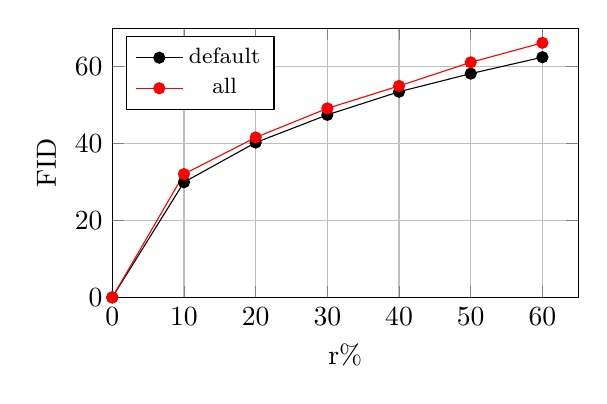
\begin{tikzpicture}
\begin{axis}[
    title={},
    height=5cm,
    width=7.5cm,
    xlabel={r\%},
    ylabel={FID},
    xmin=0, xmax=65,
    ymin=0, ymax=70,
    xtick={0,10,20,30,40,50,60},
    ytick={0,20,40,60},
    legend pos=north west,
    xmajorgrids=true,
    ymajorgrids=true,
    legend style={font=\footnotesize}
]

\addplot[
    color=black,
    mark=*
    ]
    coordinates {
    (0,0)(10,29.95)(20,40.26)(30,47.47)(40,53.48)(50,58.19)(60,62.46)
    };
    
\addplot[
    color=red,
    mark=*
    ]
    coordinates {
    (0,0)(10,32.07)(20,41.60)(30,49.15)(40,54.99)(50,61.13)(60,66.20)
    };
    
\legend{default, all}
    
\end{axis}
\end{tikzpicture}
   % time values for run2 and run3
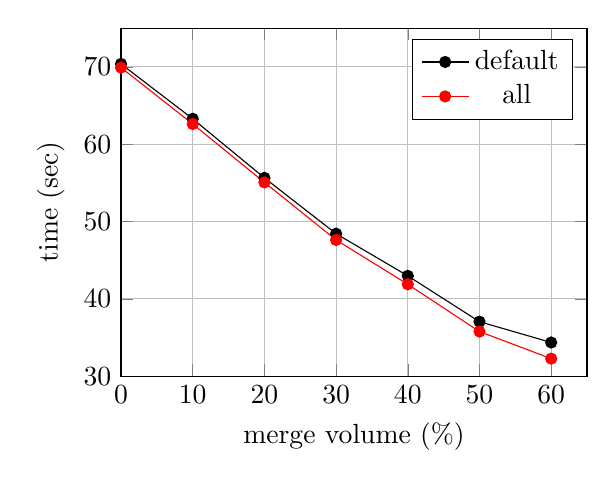
\begin{tikzpicture}
\begin{axis}[
    title={},
    height=6cm,
    width=7.5cm,
    xlabel={merge volume (\%)},
    ylabel={time (sec)},
    xmin=0, xmax=65,
    ymin=30, ymax=75,
    xtick={0,10,20,30,40,50,60},
    ytick={30,40,50,60,70},
    legend pos=north east,
    xmajorgrids=true,
    ymajorgrids=true,
]

\addplot[
    color=black,
    mark=*
    ]
    coordinates {
    (0,70.38)(10,63.28)(20,55.64)(30,48.42)(40,42.97)(50,37.04)(60,34.35)
    };
    
\addplot[
    color=red,
    mark=*
    ]
    coordinates {
    (0,69.91)(10,62.61)(20,55.06)(30,47.61)(40,41.88)(50,35.76)(60,32.26)
    };
    
\legend{default, all}
    
\end{axis}
\end{tikzpicture}
\caption{FID and time for 1.1)}
\label{fig:exp_1_1}
\end{figure}\\
This seemingly does not yield significant improvements as image generation speed does narrowly decrease by up to 2.1 s/im (this time-delta is below 1 s/im for $r<40\%$ though; see Tab.~\ref{table:exp_1_1}), albeit at a clear cost of image quality with FID being consistently larger for this configuration. \\
ToMe in its default setup consistently produces images closer to their no-ToMe original (see Fig.~\ref{fig:exp_1_1}), so extending token merging to both the cross-attn and mlp layer does not appear beneficial. This naive approach can therefore be disregarded.



%\newpage
\subsubsection*{1.2): [default] vs [self-attn \& cross-attn] vs [self-attn \& mlp]}
After \(1.1)\), the question remains whether performance drops were caused by using ToMe in both the cross-attn and mlp layer or only one of them, so the second experiment of part 1 attempts to delve deeper into that matter. This time token merging is only extended to either the cross-attn (red) or the mlp module (blue). Then a comparison is made with the results of the default ToMe settings (black) from the previous trial.
\begin{figure}[!htb]
    % FID values for run2, run4 and run5
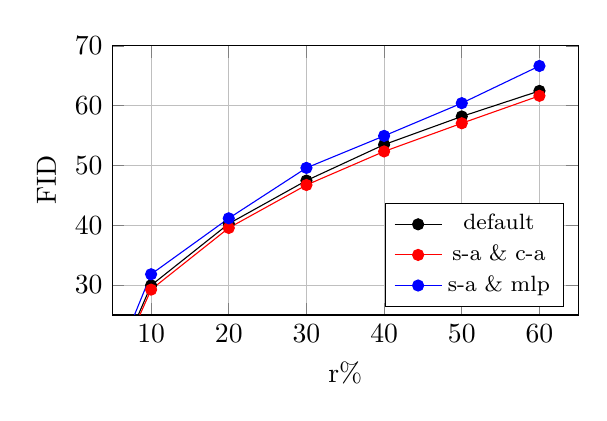
\begin{tikzpicture}
\begin{axis}[
    title={},
    height=5cm,
    width=7.5cm,
    xlabel={r\%},
    ylabel={FID},
    xmin=5, xmax=65,
    ymin=25, ymax=70,
    xtick={10,20,30,40,50,60},
    ytick={30,40,50,60,70},
    legend pos=south east,
    xmajorgrids=true,
    ymajorgrids=true,
    legend style={font=\footnotesize}
]

\addplot[
    color=black,
    mark=*
    ]
    coordinates {
    (0,0)(10,29.95)(20,40.26)(30,47.47)(40,53.48)(50,58.19)(60,62.46)
    };
    
\addplot[
    color=red,
    mark=*
    ]
    coordinates {
    (0,0)(10,29.24)(20,39.55)(30,46.73)(40,52.34)(50,57.05)(60,61.64)
    };

\addplot[
    color=blue,
    mark=*
    ]
    coordinates {
    (0,0)(10,31.81)(20,41.16)(30,49.59)(40,54.94)(50,60.41)(60,66.63)
    };
    
\legend{default, s-a \& c-a, s-a \& mlp}
    
\end{axis}
\end{tikzpicture}
    % time values for run2, run4 and run5
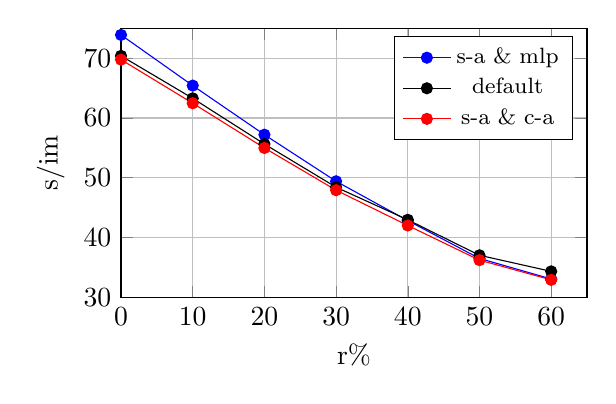
\begin{tikzpicture}
\begin{axis}[
    title={},
    height=5cm,
    width=7.5cm,
    xlabel={r\%},
    ylabel={s/im},
    xmin=0, xmax=65,
    ymin=30, ymax=75,
    xtick={0,10,20,30,40,50,60},
    ytick={30,40,50,60,70},
    legend pos=north east,
    xmajorgrids=true,
    ymajorgrids=true,
    legend style={font=\footnotesize}
]

\addplot[
    color=blue,
    mark=*
    ]
    coordinates {
    (0,73.88)(10,65.41)(20,57.20)(30,49.41)(40,42.83)(50,36.51)(60,33.08)
    };

\addplot[
    color=black,
    mark=*
    ]
    coordinates {
    (0,70.38)(10,63.28)(20,55.64)(30,48.42)(40,42.97)(50,37.04)(60,34.35)
    };
    
\addplot[
    color=red,
    mark=*
    ]
    coordinates {
    (0,69.75)(10,62.46)(20,54.98)(30,47.92)(40,42.02)(50,36.23)(60,32.93)
    };

    
\legend{s-a \& mlp, default, s-a \& c-a}
    
\end{axis}
\end{tikzpicture}
\caption{FID and time for 1.2)}
\label{fig:exp_1_2}
\end{figure}\\
This time it's clearly visible that merging tokens within the self-attn and cross-attn module performs the best, both in terms of image quality and image generation speed, notably surpassing the default configuration established by \cite{bolya2023tomesd} (see Fig.~\ref{fig:exp_1_2}).\\
Token merging in the self-attn and mlp module on the other hand noticeably worsens the image quality across the board as well as the generation speed when $r<40\%$ compared to the default (see Tab.~\ref{table:exp_1_2}).\\
We can therefore conclude that extending token merging to the cross-attn module has positive effects on the performance, while extending it to the mlp module has the opposite effect.



\newpage
\subsubsection*{1.3): [default] vs [cross-attn \& mlp] vs [only cross-attn]}
The common denominator of the previous examinations was the application of token merging in the self-attn layer. This time we are explicitly avoiding token merging in the self-attn module and instead apply it in only the cross-attn (blue) and both the cross-attn and mlp component (red).
The results of the default ToMe settings (black) again carry over from the previous trial.
\begin{figure}[!htb]
    % FID values for run8 and run9
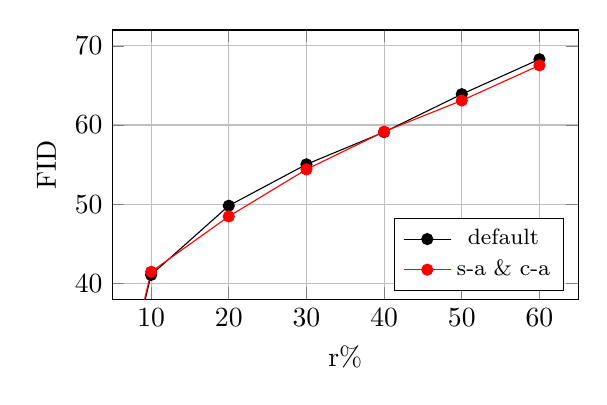
\begin{tikzpicture}
\begin{axis}[
    title={},
    height=5cm,
    width=7.5cm,
    xlabel={r\%},
    ylabel={FID},
    xmin=5, xmax=65,
    ymin=38, ymax=72,
    xtick={10,20,30,40,50,60},
    ytick={30,40,50,60,70},
    legend pos=south east,
    xmajorgrids=true,
    ymajorgrids=true,
    legend style={font=\footnotesize}
]

\addplot[
    color=black,
    mark=*
    ]
    coordinates {
    (0,0)(10,41.06)(20,49.80)(30,55.03)(40,59.10)(50,63.89)(60,68.30)
    };
    
\addplot[
    color=red,
    mark=*
    ]
    coordinates {
    (0,0)(10,41.45)(20,48.45)(30,54.39)(40,59.16)(50,63.09)(60,67.53)
    };
    
\legend{default, s-a \& c-a}
    
\end{axis}
\end{tikzpicture}
    % time values for run2, run6 and run7
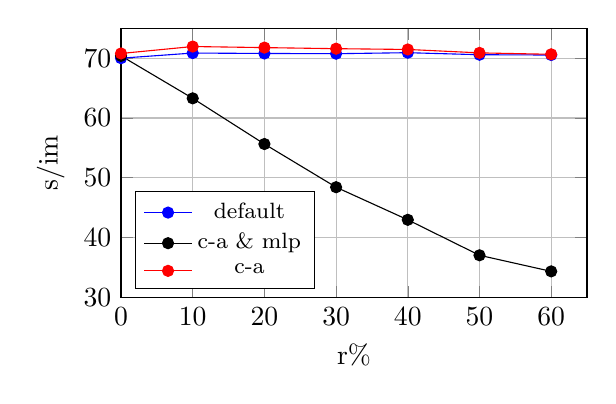
\begin{tikzpicture}
\begin{axis}[
    title={},
    height=5cm,
    width=7.5cm,
    xlabel={r\%},
    ylabel={s/im},
    xmin=0, xmax=65,
    ymin=30, ymax=75,
    xtick={0,10,20,30,40,50,60},
    ytick={30,40,50,60,70},
    legend pos=south west,
    xmajorgrids=true,
    ymajorgrids=true,
    legend style={font=\footnotesize}
]

\addplot[
    color=blue,
    mark=*
    ]
    coordinates {
    (0,69.99)(10,70.85)(20,70.78)(30,70.74)(40,70.91)(50,70.57)(60,70.52)
    };

\addplot[
    color=black,
    mark=*
    ]
    coordinates {
    (0,70.38)(10,63.28)(20,55.64)(30,48.42)(40,42.97)(50,37.04)(60,34.35)
    };
    
\addplot[
    color=red,
    mark=*
    ]
    coordinates {
    (0,70.78)(10,71.94)(20,71.76)(30,71.58)(40,71.45)(50,70.88)(60,70.64)
    };

    
\legend{default, c-a \& mlp, c-a}
    
\end{axis}
\end{tikzpicture}
\caption{FID and time for 1.3)}
\label{fig:exp_1_3}
\end{figure}\\
The most striking result here is that no token merging in the self-attn layer corresponds to no image generation speedup at all, rather slowing the process down (see Tab.~\ref{table:exp_1_3}). 
The apparent improvements to image quality compared to the ToMe default (see Fig.~\ref{fig:exp_1_3}) consequently become negligible without any speed benefits.\\
We conclusively derive that ToMe without involvement of the self-attn layer does not accelerate the image generation process at all and can be considered redundant and therefore be disregarded.




\newpage
\subsubsection*{1.4): [default] vs [self-attn \& cross-attn] (the second time)}
The most prominent takeaway of the first three experiments is that token merging in both the self-attn and cross-attn layer improves the performance of ToMe both in terms of image quality and image generation speed.\\
We now want to examine this discovery by repeating the experiment with a new set of 500 different prompt-seed-pairs and then averaging the results of both trials.
\begin{figure}[!htb]
    % FID values for run2, run6 and run7
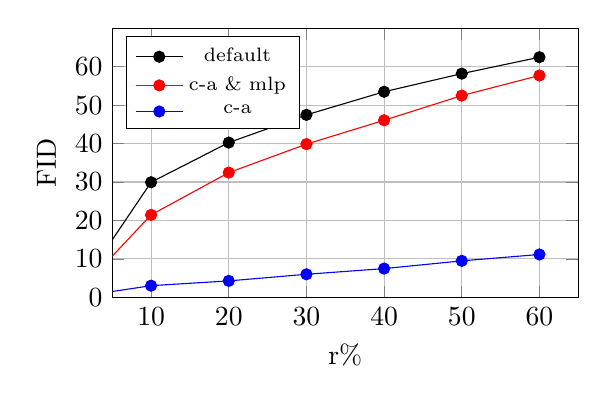
\begin{tikzpicture}
\begin{axis}[
    title={},
    height=5cm,
    width=7.5cm,
    xlabel={r\%},
    ylabel={FID},
    xmin=5, xmax=65,
    ymin=0, ymax=70,
    xtick={10,20,30,40,50,60},
    ytick={0,10,20,30,40,50,60},
    legend pos=north west,
    xmajorgrids=true,
    ymajorgrids=true,
    legend style={font=\scriptsize}
]

\addplot[
    color=black,
    mark=*
    ]
    coordinates {
    (0,0)(10,29.95)(20,40.26)(30,47.47)(40,53.48)(50,58.19)(60,62.46)
    };
    
\addplot[
    color=red,
    mark=*
    ]
    coordinates {
    (0,0)(10,21.46)(20,32.45)(30,39.86)(40,46.06)(50,52.48)(60,57.71)
    };

\addplot[
    color=blue,
    mark=*
    ]
    coordinates {
    (0,0)(10,3.05)(20,4.29)(30,6.01)(40,7.49)(50,9.50)(60,11.16)
    };

    
\legend{default, c-a \& mlp, c-a}
    
\end{axis}
\end{tikzpicture}
    % time values for run10 and run11
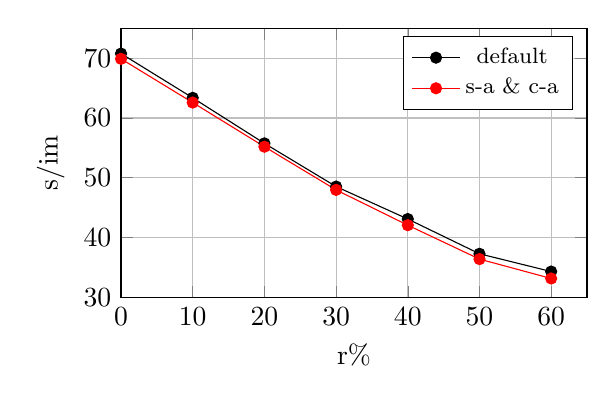
\begin{tikzpicture}
\begin{axis}[
    title={},
    height=5cm,
    width=7.5cm,
    xlabel={r\%},
    ylabel={s/im},
    xmin=0, xmax=65,
    ymin=30, ymax=75,
    xtick={0,10,20,30,40,50,60},
    ytick={30,40,50,60,70},
    legend pos=north east,
    xmajorgrids=true,
    ymajorgrids=true,
    legend style={font=\footnotesize}
]

\addplot[
    color=black,
    mark=*
    ]
    coordinates {
    (0,70.76)(10,63.36)(20,55.75)(30,48.53)(40,43.10)(50,37.29)(60,34.32)
    };
    
\addplot[
    color=red,
    mark=*
    ]
    coordinates {
    (0,69.88)(10,62.57)(20,55.19)(30,47.97)(40,42.07)(50,36.40)(60,33.16)
    };
    
\legend{default, s-a \& c-a}
    
\end{axis}
\end{tikzpicture}
\caption{FID and time for 1.4)}
\label{fig:exp_1_4}
\end{figure}\\
It is again clearly visible that token merging only in the self-attn module is outperformed by expanding it to the cross-attn module as well (see Fig.~\ref{fig:exp_1_4}).
\\
Note that FID doesn’t consider prompt adherance, which is likely why merging the cross attn module actually reduces FID. (Still relevent with different expermient setup??)



\newpage
\subsubsection*{2): Exploring different images sizes}
Text.
\subsubsection*{2.1): Moving to smaller images}
Test1
\begin{figure}[!htb]
    % FID values for run8 and run9
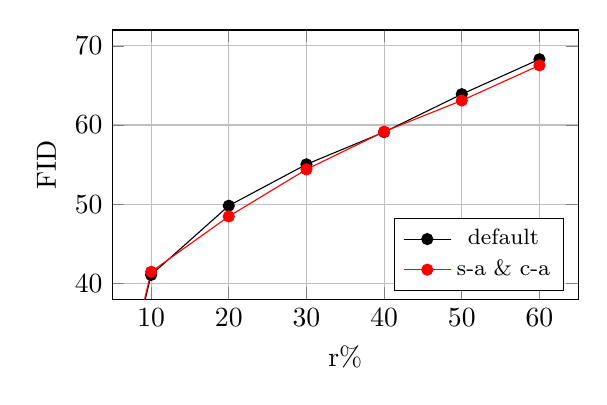
\begin{tikzpicture}
\begin{axis}[
    title={},
    height=5cm,
    width=7.5cm,
    xlabel={r\%},
    ylabel={FID},
    xmin=5, xmax=65,
    ymin=38, ymax=72,
    xtick={10,20,30,40,50,60},
    ytick={30,40,50,60,70},
    legend pos=south east,
    xmajorgrids=true,
    ymajorgrids=true,
    legend style={font=\footnotesize}
]

\addplot[
    color=black,
    mark=*
    ]
    coordinates {
    (0,0)(10,41.06)(20,49.80)(30,55.03)(40,59.10)(50,63.89)(60,68.30)
    };
    
\addplot[
    color=red,
    mark=*
    ]
    coordinates {
    (0,0)(10,41.45)(20,48.45)(30,54.39)(40,59.16)(50,63.09)(60,67.53)
    };
    
\legend{default, s-a \& c-a}
    
\end{axis}
\end{tikzpicture}
    % time values for run8 and run9
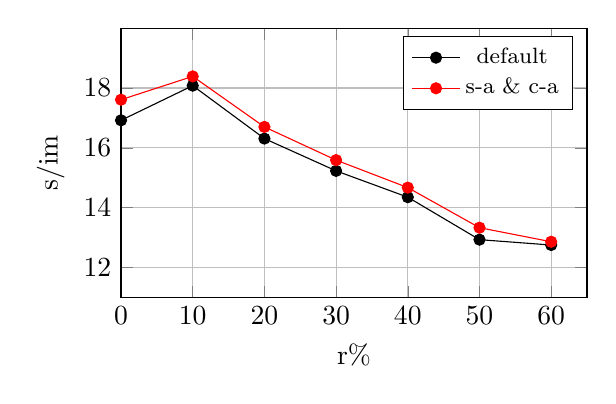
\begin{tikzpicture}
\begin{axis}[
    title={},
    height=5cm,
    width=7.5cm,
    xlabel={r\%},
    ylabel={s/im},
    xmin=0, xmax=65,
    ymin=11, ymax=20,
    xtick={0,10,20,30,40,50,60},
    ytick={12,14,16,18},
    legend pos=north east,
    xmajorgrids=true,
    ymajorgrids=true,
    legend style={font=\footnotesize}
]

\addplot[
    color=black,
    mark=*
    ]
    coordinates {
    (0,16.92)(10,18.08)(20,16.31)(30,15.23)(40,14.35)(50,12.93)(60,12.75)
    };
    
\addplot[
    color=red,
    mark=*
    ]
    coordinates {
    (0,17.61)(10,18.39)(20,16.70)(30,15.59)(40,14.67)(50,13.33)(60,12.86)
    };
    
\legend{default, s-a \& c-a}
    
\end{axis}
\end{tikzpicture}
\end{figure}



\newpage
\subsubsection*{3): Exploring different strides}
\subsubsection*{3.1): $3 \times 3$ stride}
Test1
\subsubsection*{3.2): $1 \times 2$ vertical stride}
\begin{align*}
    r_{max} = 1-\frac{1}{1*2} = 50\%
\end{align*}
Every  \textbf{src} token has to merged when \(r=50\%\) because \(r=r_{max}\) now so the advantage starts to fade.

\begin{figure}[!htb]
    % FID values for run11, run14 and run15 
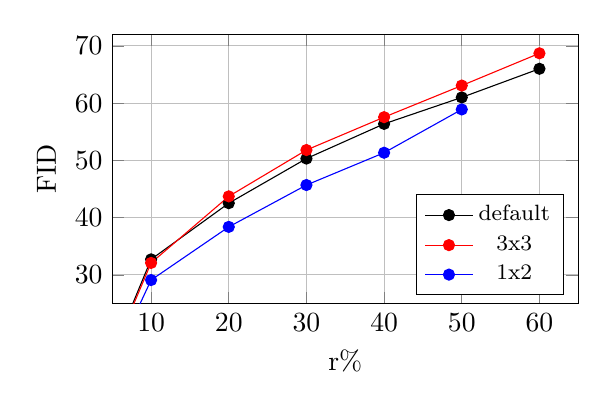
\begin{tikzpicture}
\begin{axis}[
    title={},
    height=5cm,
    width=7.5cm,
    xlabel={r\%},
    ylabel={FID},
    xmin=5, xmax=65,
    ymin=25, ymax=72,
    xtick={10,20,30,40,50,60},
    ytick={30,40,50,60,70},
    legend pos=south east,
    xmajorgrids=true,
    ymajorgrids=true,
    legend style={font=\footnotesize}
]

\addplot[
    color=black,
    mark=*
    ]
    coordinates {
    (0,0)(10,32.71)(20,42.52)(30,50.31)(40,56.37)(50,60.99)(60,65.99)
    };
    
\addplot[
    color=red,
    mark=*
    ]
    coordinates {
    (0,0)(10,32.09)(20,43.71)(30,51.80)(40,57.54)(50,63.06)(60,68.69)
    };

\addplot[
    color=blue,
    mark=*
    ]
    coordinates {
    (0,0)(10,29.10)(20,38.38)(30,45.69)(40,51.33)(50,58.89)
    };
    
\legend{default, 3x3, 1x2}
    
\end{axis}
\end{tikzpicture}
    % time values for run11, run14 and run15
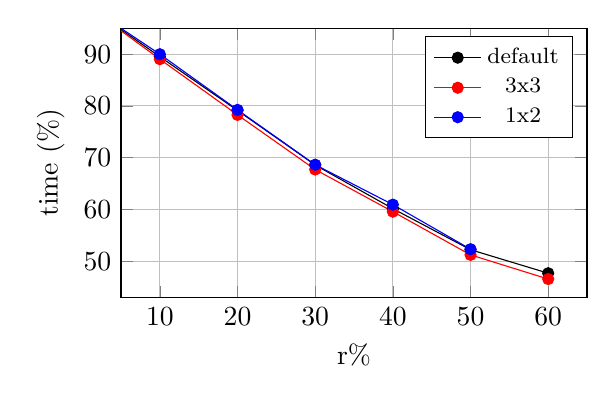
\begin{tikzpicture}
\begin{axis}[
    title={},
    height=5cm,
    width=7.5cm,
    xlabel={r\%},
    ylabel={time (\%)},
    xmin=5, xmax=65,
    ymin=43, ymax=95,
    xtick={10,20,30,40,50,60},
    ytick={50,60,70,80,90},
    legend pos=north east,
    xmajorgrids=true,
    ymajorgrids=true,
    legend style={font=\footnotesize}
]

\addplot[
    color=black,
    mark=*
    ]
    coordinates {
    (0,100)(10,89.50)(20,79.11)(30,68.57)(40,60.14)(50,52.21)(60,47.67)
    };
    
\addplot[
    color=red,
    mark=*
    ]
    coordinates {
    (0,100)(10,89.02)(20,78.26)(30,67.70)(40,59.56)(50,51.21)(60,46.54)
    };

\addplot[
    color=blue,
    mark=*
    ]
    coordinates {
    (0,100)(10,89.98)(20,79.23)(30,68.63)(40,60.92)(50,52.31)
    };
    
\legend{default, 3x3, 1x2}
    
\end{axis}
\end{tikzpicture}
\end{figure}



\newpage
\subsubsection*{4): Putting it all together}
Averages of default by \cite{bolya2023tomesd}, improvement by using selt-attn and cross-attn, improvement by using 1x2 strides. 
self-attn and cross-attn with 2x2 strides for best time performance. self-attn and cross-attn with 1x2 strides for best quality (low FID) performance.
\begin{figure}[!htb]
    % FID values for run2/10, run4/11 and run15/16
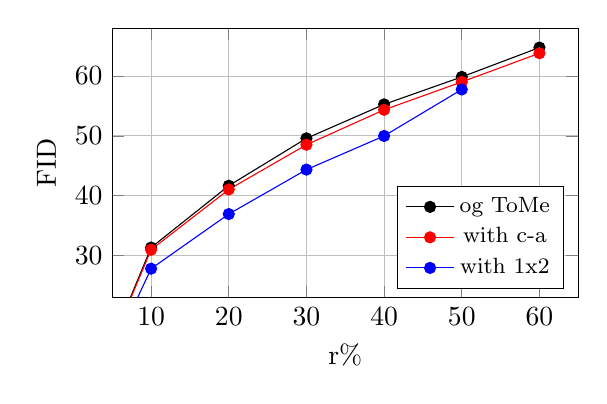
\begin{tikzpicture}
\begin{axis}[
    title={},
    height=5cm,
    width=7.5cm,
    xlabel={r\%},
    ylabel={FID},
    xmin=5, xmax=65,
    ymin=23, ymax=68,
    xtick={10,20,30,40,50,60},
    ytick={30,40,50,60},
    legend pos=south east,
    xmajorgrids=true,
    ymajorgrids=true,
    legend style={font=\footnotesize}
]

\addplot[
    color=black,
    mark=*
    ]
    coordinates {
    (0,0)(10,31.33)(20,41.67)(30,49.59)(40,55.27)(50,59.86)(60,64.77)
    };
    
\addplot[
    color=red,
    mark=*
    ]
    coordinates {
    (0,0)(10,30.97)(20,41.04)(30,48.52)(40,54.36)(50,59.02)(60,63.82)
    };

\addplot[
    color=blue,
    mark=*
    ]
    coordinates {
    (0,0)(10,27.80)(20,36.93)(30,44.36)(40,49.99)(50,57.76)
    };
    
\legend{og ToMe, with c-a, with 1x2}
    
\end{axis}
\end{tikzpicture}
    % time values for run2/10, run4/11, run15/16
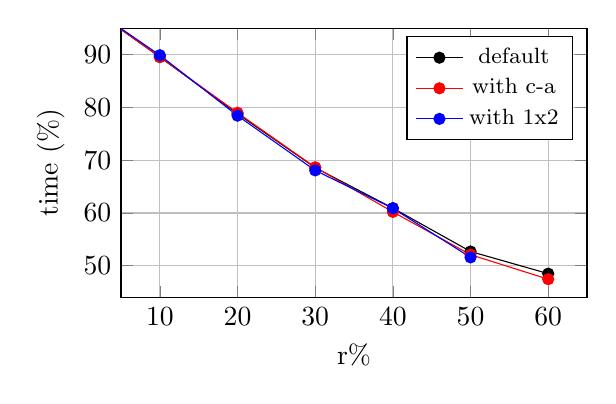
\begin{tikzpicture}
\begin{axis}[
    title={},
    height=5cm,
    width=7.5cm,
    xlabel={r\%},
    ylabel={time (\%)},
    xmin=5, xmax=65,
    ymin=44, ymax=95,
    xtick={10,20,30,40,50,60},
    ytick={50,60,70,80,90},
    legend pos=north east,
    xmajorgrids=true,
    ymajorgrids=true,
    legend style={font=\footnotesize}
]

\addplot[
    color=black,
    mark=*
    ]
    coordinates {
    (0,100)(10,89.54)(20,78.79)(30,68.58)(40,60.91)(50,52.70)(60,48.50)
    };
    
\addplot[
    color=red,
    mark=*
    ]
    coordinates {
    (0,100)(10,89.54)(20,78.98)(30,68.65)(40,60.20)(50,52.09)(60,47.45)
    };

\addplot[
    color=blue,
    mark=*
    ]
    coordinates {
    (0,100)(10,89.89)(20,78.43)(30,68.06)(40,60.88)(50,51.58)
    };
    
\legend{default, with c-a, with 1x2}
    
\end{axis}
\end{tikzpicture}
\end{figure}



\subsubsection*{Summary}